\begin{enumerate}[label=(\alph*)]
    \item Make a Venn diagram for the sets $(A \cup B) \mybackslash C$ and $A \cup (B \mybackslash C)$. What can you conclude about whether one of these sets is necessarily, a subset of the other?
    \item Give an example of sets $A,B,$ and $C$ for which $(A \cup B) \mybackslash C \neq A \cup (B \mybackslash C)$.
\end{enumerate}

\textbf{Solution:}
\begin{enumerate}[label=(\alph*)]
    \item We first draw $A \cup (B \mybackslash C)$ below. \\
    
    \
    
        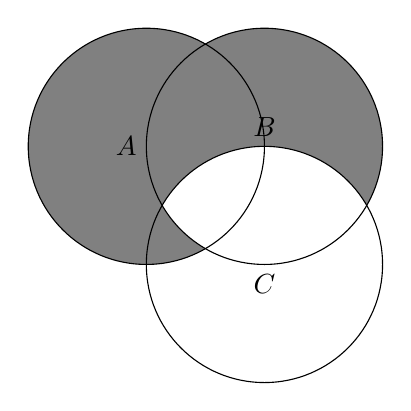
\begin{tikzpicture}
          % Define circles for A, B, and C
          \def\circleA{(0,0) circle (1.5cm)}
          \def\circleB{(1.5,0) circle (1.5cm)}
          \def\circleC{(1.5,-1.5) circle (1.5cm)}
        
          % Fill A
          \begin{scope}
            \fill[gray] \circleA;
          \end{scope}
        
          % Fill B excluding C
          \begin{scope}
            \clip \circleB;
            \fill[gray] \circleB;
            \clip \circleC;
            \fill[white] \circleB;
          \end{scope}
        
          % Outline the circles and label them
          \draw \circleA node [text=black, left] {$A$};
          \draw \circleB node [text=black, above] {$B$};
          \draw \circleC node [text=black, below] {$C$};
        \end{tikzpicture}

    Next, we draw $(A \cup B) \mybackslash C$ below. \\
    
    \
    
        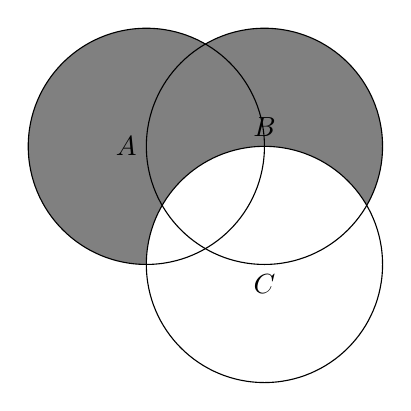
\begin{tikzpicture}
          % Define circles for A, B, and C
          \def\circleA{(0,0) circle (1.5cm)}
          \def\circleB{(1.5,0) circle (1.5cm)}
          \def\circleC{(1.5,-1.5) circle (1.5cm)}
        
          % Fill A
          \begin{scope}
            \fill[gray] \circleA;
            \clip \circleC;
            \fill[white] \circleC;
          \end{scope}
        
          % Fill B excluding C
          \begin{scope}
            \clip \circleB;
            \fill[gray] \circleB;
            \clip \circleC;
            \fill[white] \circleB;
          \end{scope}
        
          % Outline the circles and label them
          \draw \circleA node [text=black, left] {$A$};
          \draw \circleB node [text=black, above] {$B$};
          \draw \circleC node [text=black, below] {$C$};
        \end{tikzpicture}

    Note that in $A \cup (B \mybackslash C)$, $A \cap C$ is nonempty. Meanwhile in $(A \cup B) \mybackslash C$ the set $A \cap C$ is empty. Everything else is equivalent. Hence, $(A \cup B) \mybackslash C \subseteq A \cup (B \mybackslash C)$.
    
    \item Let $A=\{1,2,3\}$, $B=\{3,4,5\}$ and $C=\{1,5\}$. Now, $(A \cup B) \setminus C$ gives us $\{1, 2, 3, 4, 5\} \setminus \{1, 5\} = \{2, 3, 4\}$, while $A \cup (B \setminus C)$ gives us $\{1, 2, 3\} \cup \{3, 4\} = \{1, 2, 3, 4\}$. These two results are clearly different: $\{2, 3, 4\} \neq \{1, 2, 3, 4\}$. This example correctly illustrates the inequality between $(A \cup B) \setminus C$ and $A \cup (B \setminus C)$.
\end{enumerate}
\pagebreak